% TikZ schematic: FFT Feature Extraction Pipeline (Tutorial 1)
% Compile: pdflatex t01_fft_pipeline.tex
\documentclass[border=10pt]{standalone}
\usepackage{tikz}
\usepackage{xcolor}
\usetikzlibrary{shapes,arrows,positioning,calc,decorations.pathreplacing,patterns,fit,backgrounds}

\definecolor{inputblue}{RGB}{31,119,180}
\definecolor{fftgreen}{RGB}{44,160,44}
\definecolor{featorange}{RGB}{255,127,14}
\definecolor{arrowgray}{RGB}{100,100,100}

\begin{document}
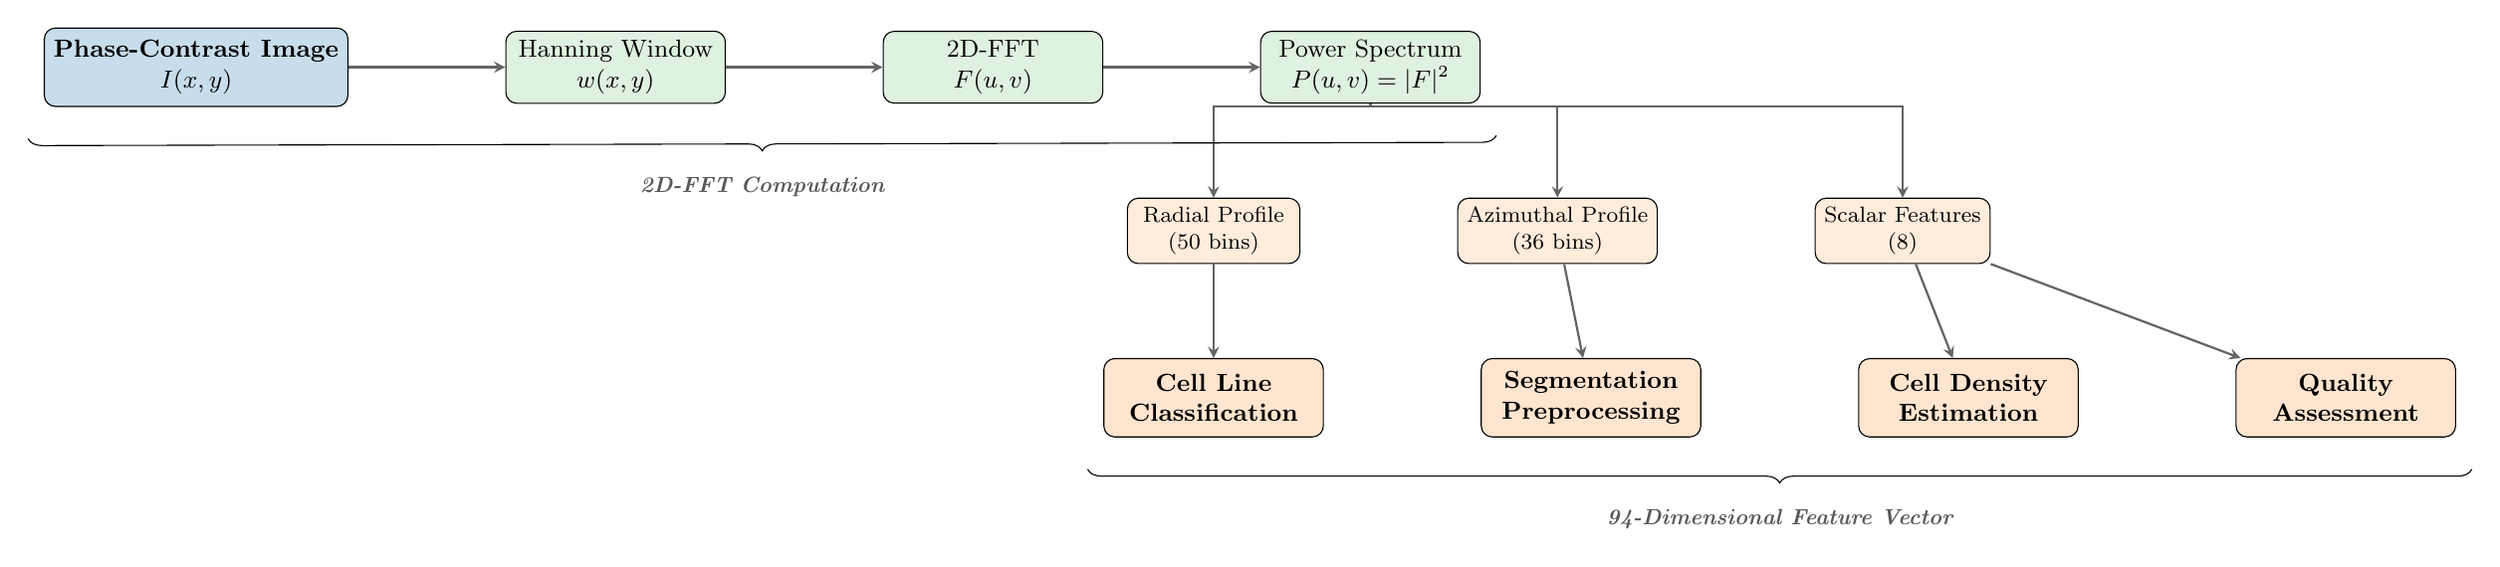
\begin{tikzpicture}[
    node distance=1.5cm and 2cm,
    box/.style={rectangle, draw, rounded corners, fill=inputblue!15, minimum width=2.8cm, minimum height=1cm, align=center, font=\small\bfseries},
    proc/.style={rectangle, draw, rounded corners, fill=fftgreen!15, minimum width=2.8cm, minimum height=0.8cm, align=center, font=\small},
    feat/.style={rectangle, draw, rounded corners, fill=featorange!15, minimum width=2.2cm, minimum height=0.7cm, align=center, font=\footnotesize},
    arrow/.style={->, >=stealth, thick, color=arrowgray},
    label/.style={font=\footnotesize\itshape, color=gray!70!black}
]

% Row 1: Main pipeline
\node[box, fill=inputblue!25] (input) {Phase-Contrast Image\\$I(x,y)$};
\node[proc, right=of input] (window) {Hanning Window\\$w(x,y)$};
\node[proc, right=of window] (fft) {2D-FFT\\$F(u,v)$};
\node[proc, right=of fft] (psd) {Power Spectrum\\$P(u,v)=|F|^2$};

% Row 2: Feature extraction
\node[feat, below=1.2cm of psd, xshift=-2cm] (radial) {Radial Profile\\(50 bins)};
\node[feat, right=of radial] (azimuth) {Azimuthal Profile\\(36 bins)};
\node[feat, right=of azimuth] (scalar) {Scalar Features\\(8)};

% Row 3: Applications
\node[box, fill=featorange!20, below=1.2cm of radial] (class) {Cell Line\\Classification};
\node[box, fill=featorange!20, right=of class] (seg) {Segmentation\\Preprocessing};
\node[box, fill=featorange!20, right=of seg] (density) {Cell Density\\Estimation};
\node[box, fill=featorange!20, right=of density] (quality) {Quality\\Assessment};

% Arrows
\draw[arrow] (input) -- (window);
\draw[arrow] (window) -- (fft);
\draw[arrow] (fft) -- (psd);

\draw[arrow] (psd) -- ++(0,-0.5) -| (radial);
\draw[arrow] (psd) -- ++(0,-0.5) -| (azimuth);
\draw[arrow] (psd) -- ++(0,-0.5) -| (scalar);

\draw[arrow] (radial) -- (class);
\draw[arrow] (azimuth) -- (seg);
\draw[arrow] (scalar) -- (density);
\draw[arrow] (scalar) -- (quality);

% Braces
\draw[decorate, decoration={brace, amplitude=5pt, mirror, raise=3pt}]
    ($(input.south west)+(-0.2,-0.3)$) -- ($(psd.south east)+(0.2,-0.3)$)
    node[midway, below=0.5cm, label] {\textbf{2D-FFT Computation}};

\draw[decorate, decoration={brace, amplitude=5pt, mirror, raise=3pt}]
    ($(class.south west)+(-0.2,-0.3)$) -- ($(quality.south east)+(0.2,-0.3)$)
    node[midway, below=0.5cm, label] {\textbf{94-Dimensional Feature Vector}};

\end{tikzpicture}
\end{document}
